% =============================================
% =============================================
% Document class: Article
\documentclass[ a4paper, twoside, 11pt]{article}
% Packages: LaTeX (Depth-1)
\usepackage[ vlined, linesnumbered, ruled]{algorithm2e}
\usepackage{ amsfonts, amsmath, amssymb, amsthm}
\usepackage[ titletoc, title]{appendix}
\usepackage{ bbm}
\usepackage{ color}
\usepackage{ dsfont}
\usepackage{ enumitem}
\usepackage{ graphicx}
\usepackage{ fancyhdr, float, fullpage}
\usepackage{ hyperref}
\usepackage{ lastpage, latexsym, lipsum}
\usepackage{ mathrsfs, mathtools, multicol}
\usepackage{ parskip}
\usepackage{ setspace, stmaryrd, subcaption}
\usepackage{ tabularx}
\usepackage{ wasysym}
\usepackage[ dvipsnames, table]{ xcolor}
\usepackage{ xfrac}
% Packages: LaTeX (Depth-2)
\usepackage{ epstopdf}

% =============================================
\topmargin 			= -1.6cm
\headheight 		= .90cm
\headsep 			= .80cm
\textheight 		= 24.0cm
\textwidth 			= 15.5cm
\oddsidemargin		= 0.cm
\evensidemargin 	= 0.cm

% =============================================
% =============================================
% Macros: Language
\newcommand{\define}{\triangleq}
\newcommand{\done}{\hfill $\square$}
%\newcommand{\eqCIRC}{\stackrel{\circ}{=}}
%\newcommand{\eqSTAR}{\stackrel{*}{=}}
\renewcommand{\epsilon}{\varepsilon}
\newcommand{\eg}{\textit{e.g.,\;}}
\newcommand{\egc}{\textit{e.g.:\;}}
\newcommand{\Eg}{\textit{E.g.,\;}}
\newcommand{\Egc}{\textit{E.g.:\;}}
\newcommand{\ie}{\textit{i.e.,\;}}
\newcommand{\iec}{\textit{i.e.:\;}}
\newcommand{\Ie}{\textit{I.e.,\;}}
\newcommand{\Iec}{\textit{I.e.:\;}}
\newcommand{\QED}{\hfill $\blacksquare$}
\renewcommand{\tilde}[1]{\widetilde{#1}}
\newcommand{\tsup}[1]{\ensuremath{^{\text{#1}}}}
\newcommand{\tsub}[1]{\ensuremath{_{\text{#1}}}}
\renewcommand{\vec}[1]{{\boldsymbol{#1}}}

% Macros: Optimization & Probability
\DeclareMathOperator*{\argmax}{arg\,max}
\DeclareMathOperator*{\argmin}{arg\,min}
\newcommand{\Exp}{\mathbb{E}}
\newcommand{\Indicate}[1]{ \IndFun \, \{ \, #1 \, \} }
\renewcommand{\Pr}{\mathbb{P}}
\newcommand{\Normal}{\mathcal{N}}
\newcommand{\std}{\text{std}}
\newcommand{\var}{\text{var}}

% Macros: Sets
\newcommand{\Complex}{\mathbb{C}}
\renewcommand{\emptyset}{\varnothing}
\newcommand{\Nat}{\mathbb{N}}
\renewcommand{\Re}{\mathbb{R}}
\newcommand{\ReNN}{{\Re}_{\geq 0}}
\newcommand{\ReSP}{{\Re}_{> 0}}
\renewcommand{\subset}{\subseteq}
\renewcommand{\supset}{\supseteq}
\newcommand{\Z}{\mathbb{Z}}
\newcommand{\ZNN}{{\Z}_{\geq 0}}

% Macros: Spacing & Other Commands
\newcommand{\fullcut}{\vspace{-\baselineskip}}
\newcommand{\fullskip}{\vspace{\baselineskip}}
\newcommand{\halfcut}{\vspace{-0.5\baselineskip}}
\newcommand{\halfskip}{\vspace{0.5\baselineskip}}
\renewcommand{\figurename}{Figura}
\renewcommand{\tablename}{Tabla}

% =============================================
% Sesion de Clase
\newcommand{\sesion}{03}
% Macros para definiciones, teoremas, etc
\newcounter{sesion}
\setcounter{sesion}{\sesion}
\theoremstyle{definition}
\newtheorem{definition}{Definici\'on}[sesion]
\newtheorem{example}[definition]{Ejemplo}
\newtheorem{exercise}[definition]{Ejercicio}
\newtheorem{note}[definition]{Nota}
\newtheorem{problem}[definition]{Problema}
\newtheorem{theorem}[definition]{Teorema}

% =============================================
% =============================================
\newcommand{\HeaderLine}{}
\newcommand{\FooterLine}{P\'agina \thepage ~de \pageref*{LastPage}}

\pagestyle{fancyplain}
\fancyhf{}

\rhead[]{\fancyplain{}{\HeaderLine}}
\lhead[\fancyplain{}{\HeaderLine}]{}
\lfoot[\fancyplain{}{\FooterLine}]{}
\rfoot[]{\fancyplain{}{\FooterLine}}

\renewcommand{\headrulewidth}{0.4pt}
\renewcommand{\footrulewidth}{0.4pt}
\renewcommand{\thefootnote}{\fnsymbol{footnote}}

% =============================================
% =============================================
\begin{document}
\allowdisplaybreaks

\begin{center}
\Large Din\'amica (FIMCP-01271): Lecci\'on \sesion \\[0.5ex]
\small \textbf{A\~no:} 2016-2017 \qquad \textbf{T\'ermino:} II \qquad
\textbf{Instructor:} Luis I. Reyes Castro \qquad \textbf{Paralelo:} 02
\end{center}
\halfskip

\fbox{

\begin{minipage}[b][\height][t]{\textwidth}
\vspace{0.2 cm}

\begin{center}
\textbf{COMPROMISO DE HONOR}
\end{center}
\vspace{0.4 cm}

\scriptsize
{
Yo, \rule{60mm}{.1pt} al firmar este compromiso, reconozco que la presente lecci\'on est\'a dise\~nada para ser resuelta de manera individual, que puedo usar un l\'apiz o pluma y una calculadora cient\'ifica, \linebreak que solo puedo comunicarme con la persona responsable de la recepci\'on de la lecci\'on, y que cualquier instrumento de comunicaci\'on que hubiere tra\'ido debo apagarlo. Tambi\'en estoy conciente que no debo consultar libros, notas, \linebreak ni materiales did\'acticos adicionales a los que el instructor entregue durante la lecci\'on o autorice a utilizar. Finalmente, me comprometo a desarrollar y presentar mis respuestas de manera clara y ordenada. \\

Firmo al pie del presente compromiso como constancia de haberlo le\'ido y aceptado. 
\vspace{0.4 cm}

Firma: \rule{60mm}{.1pt} \qquad N\'umero de matr\'icula: \rule{40mm}{.1pt} \hspace{0.5cm} \\[-0.8ex]

}

\end{minipage}

}
\fullskip

\begin{figure}[htb]
\centering
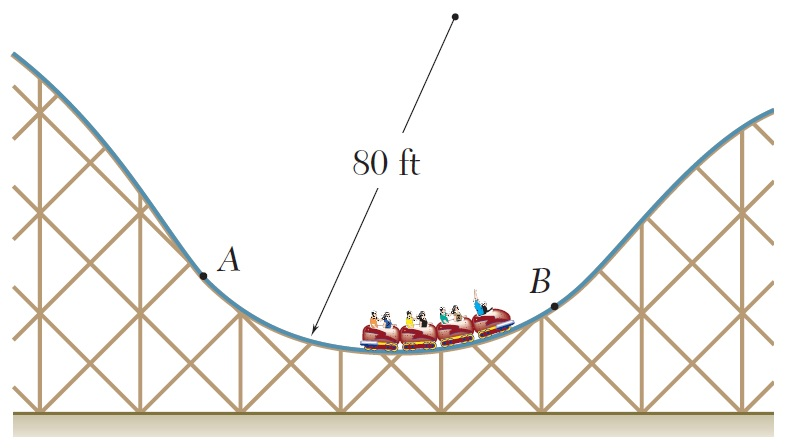
\includegraphics[ width = 0.50\textwidth]{fig_P11-136.jpg}
\qquad
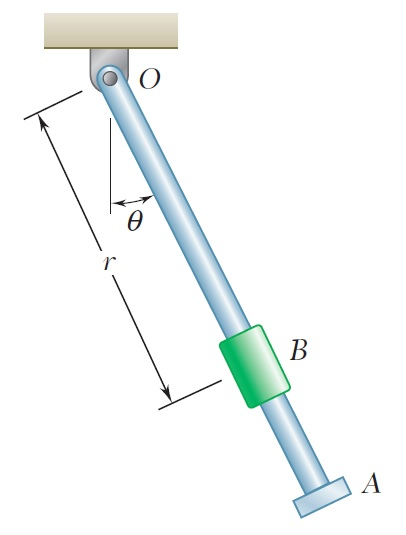
\includegraphics[ width = 0.30\textwidth]{fig_P11-164.jpg}
\end{figure}
\fullskip

% =============================================
\begin{problem}
Determine la rapidez m\'axima que los carros de la monta\~na rusa pueden alcanzar a lo largo de la porci\'on circular $AB$ de la pista, si la componente normal de su aceleraci\'on no puede ser mayor que $3g$. \textbf{[4 Puntos]}

\emph{Soluci\'on:} Mientras el carro pasa por la porci\'on $AB$ de la pista tenemos que: 
\[
a_n \, = \, \frac{v^2}{\rho}
\]
Dado que $a_n \leq 3g$ debe ser el caso que: 
\[
\frac{v^2}{\rho} \, \leq \, 3 \, g \quad \Longrightarrow \quad v \, \leq \, \sqrt{ 3 \, g \, \rho } \quad \Longrightarrow \quad v \, \leq \, 87.9 \text{ ft/s }
\]

\end{problem}
\vspace{\baselineskip}

% =============================================
\begin{problem}
La oscilaci\'on de la varilla $OA$ alrededor de $O$ se define por medio de la relaci\'on $\theta(t) = (2/\pi) \sin ( \pi t )$, donde $\theta$ y $t$ se expresan en radianes y segundos, respectivamente. El collar\'in $B$ se desliza a lo largo de la varilla de manera que su distancia desde $O$ es $r(t) = 25 / ( t + 4 )$, donde $r$ y $t$ se expresan en pulgadas y segundos, respectivamente. Cuando $t = 1$ s, encuentre: 
\begin{enumerate}[label=\alph*.]
\item \textbf{[2 Puntos]} La velocidad del collar\'in $B$. \\[1ex] \emph{Soluci\'on:} Dado que 
\[
r(t) \, = \, \frac{25}{t+4} \qquad \qquad 
\theta(t) \, = \, \left( \frac{2}{\pi} \right) \sin( \pi t )
\]
tenemos que $r(1) = 5$ in, que $\theta(1) = 0$ rad, y que: 
\begin{align*}
& \dot{r}(t) \, = \, -\frac{25}{(t+4)^2} \quad \Longrightarrow \quad \dot{r}(1) \, = \, -1 \text{ in/s} \\
& \dot{\theta}(t) \, = \, 2 \, \cos( \pi t ) \quad \Longrightarrow \quad \dot{\theta}(1) \, = \, -2 \text{ rad/s}
\end{align*}
Consecuentemente, recordando que 
\[
\vec{v}(t) \, = \, \dot{r}(t) \, \vec{\hat{e}_r}(t) + r(t) \, \dot{\theta}(t) \, \vec{\hat{e}_{\theta}}(t)
\]
concluimos que: 
\[
\vec{v}(1) \, = \, -1 \, \vec{\hat{e}_r}(1) - 10 \, \vec{\hat{e}_{\theta}}(1) \; \text{ in/s}
\]

\item \textbf{[2 Puntos]} La aceleraci\'on del collar\'in $B$. \\[1ex] \emph{Soluci\'on:} Dado que 
\[
\dot{r}(t) \, = \, -\frac{25}{(t+4)^2} \qquad \qquad 
\dot{\theta}(t) \, = \, 2 \, \cos( \pi t )
\]
vemos que: 
\begin{align*}
& \ddot{r}(t) \, = \, \frac{50}{(t+4)^3} \quad \Longrightarrow \quad \ddot{r}(1) \, = \, \frac{2}{5} \text{ in/s\tsup{2}} \, = \, 0.4 \text{ in/s\tsup{2}} \\
& \ddot{\theta}(t) \, = \, -2 \, \pi \, \sin( \pi t ) \quad \Longrightarrow \quad \ddot{\theta}(1) \, = \, 0 \text{ rad/s\tsup{2}}
\end{align*}
Consecuentemente, recordando que 
\[
\vec{a}(t) \, = \, ( \, \ddot{r}(t) - r(t) \, [\dot{\theta}(t)]^2 \, ) \, \vec{\hat{e}_r}(t) + ( \, r(t) \, \ddot{\theta}(t) + 2 \, \dot{r}(t) \, \dot{\theta}(t) \, ) \, \vec{\hat{e}_{\theta}}(t)
\]
concluimos que: 
\begin{align*}
\vec{a}(1) \, 
& = \, -\frac{98}{5} \, \vec{\hat{e}_r}(1) + 4 \, \vec{\hat{e}_{\theta}}(1) \; \text{ in/s\tsup{2}} \\[1ex]
& = \, -19.6 \, \vec{\hat{e}_r}(1) + 4 \, \vec{\hat{e}_{\theta}}(1) \; \text{ in/s\tsup{2}}
\end{align*}

\item \textbf{[2 Puntos]} La aceleraci\'on del collar\'in $B$ relativa a la varilla $OA$. \\[1ex] \emph{Soluci\'on:} Es evidente que: 
\[
a_{B/OA}(t) \, = \, \ddot{r}(t) \quad \Longrightarrow \quad a_{B/OA}(1) \, = \, \frac{2}{5} \text{ in/s\tsup{2}} \, = \, 0.4 \text{ in/s\tsup{2}}
\]
\end{enumerate}

\end{problem}
\vspace{\baselineskip}

\end{document}
